\chapter{Landasan Teori}

\section{JSON}

JSON (\textit{JavaScript Object Notation}) adalah format pertukaran data berbasis teks yang ringan dan tidak terikat pada bahasa tertentu\cite{rfc7159}. Format JSON diturunkan dari bahasa pemrograman \textit{ECMAScript}\footnote{Sering juga dikenal dengan nama \textit{JavaScript}}.

Sebuah data JSON bisa berupa salah satu dari 5 elemen berikut:

\begin{enumerate}
	\item \textbf{nilai literal}, yaitu salah satu dari ``\texttt{false}'', ``\texttt{null}'', atau ``\texttt{true}'' (tanpa tanda kutip).
	\item \textbf{bilangan}, berupa bilangan bulat maupun desimal, dengan tanda titik (``\texttt{.}'' sebagai pemisah antara bilangan bulat dengan pecahan.
	\item \textbf{\textit{string}}, deretan karakter yang diapit dengan tanda kutip ganda (``\verb/"/''). Di dalamnya bisa terdapat karakter karakter khusus seperti \textit{line feed} (``\verb/\n/''), tanda kutip ganda secara literal (``\verb/\"/''), atau garis miring terbalik secara literal (``\verb/\\/'').
	\item \textbf{larik}, nol atau lebih data JSON, yang dipisahkan koma (``\verb/,/'') dan diapit dengan kurung siku (``\verb/[/'' dan ``\verb/]/''). Data dalam \textit{array} tidak harus berjenis sama.
	\item \textbf{objek}, nol atau lebih pasangan nama/nilai, yaitu \textit{string} teks dan data JSON yang dipisahkan dengan tanda titik dua (``\verb/:/''). Untuk memisahkan pasangan satu dengan lainnya, digunakan tanda koma (``\verb/,/'').
\end{enumerate}

Data JSON dapat mengandung karakter-karakter \textit{whitespace} berupa spasi, \textit{tab}, maupun \textit{linefeed} dan akan diabaikan (kecuali di dalam \textit{string}).

Berikut adalah contoh sebuah data JSON:

\begin{lstlisting}
{
	"lulus": false,
	"nilaiUTS": 89.9,
	"nilaiUAS": null,
	"nilaiTugas": [75, null, 80.3, 100],
	"nama": "Pascal"
}
\end{lstlisting}

Contoh di atas mendemonstrasikan sebuah objek (baris 1-7), nilai literal (baris 2 dan 4), bilangan (baris 3), larik (baris 5), dan \textit{string} (baris 6).

\section{GeoJSON}

GeoJSON adalah sebuah format berbasis JSON, untuk mengkodekan berbagai struktur data geografis\cite{geojson}. Sebuah data GeoJSON selalu terdiri dari satu buah objek, yang memiliki aturan-aturan sebagai berikut:

\begin{enumerate}
	\item Objek GeoJSON dapat memiliki berapapun jumlah anggota (pasangan nama / nilai).
	\item Objek GeoJSON harus memiliki anggota, dengan nama ``\texttt{type}'', yang menunjukkan tipe dari objek GeoJSON tersebut.
	\item Nilai dari \texttt{type} harus berupa salah satu dari ``\texttt{Point}'', ``\texttt{MultiPoint}'', ``\texttt{LineString}'', ``\texttt{MultiLineString}'', ``\texttt{Polygon}'', ``\texttt{MultiPolygon}'', ``\texttt{GeometryCollection}'', ``\texttt{Feature}'', atau ``\texttt{FeatureCollection}'' (\textit{case sensitive}). Anggota ini menunjukkan tipe dari objek GeoJSON.
	\item Objek GeoJSON dapat memiliki anggota dengan nama ``\texttt{crs}'' yang menunjukkan referensi sistem koordinat.
	\item Objek GeoJSON dapat memiliki anggota dengan nama ``\texttt{bbox}'' yang menunjukkan \textit{bounding box} (kotak yang melingkupi objek).
\end{enumerate}

Subbab-subbab berikut menjelaskan bagian-bagian dari GeoJSON yang terkait dengan penelitian ini. Bagian lain yang tidak dijelaskan dapat dilihat pada \cite{geojson}.

\subsection{\textit{Geometry Object}}

\textit{Geometry Object} adalah objek-objek geometri, yaitu salah satu dari \textit{Point}, \textit{MultiPoint}, \textit{LineString}, \textit{MultiLineString}, \textit{Polygon}, \textit{MultiPolygon} atau \textit{GeometryCollection}.

Sebuah \textit{Geometry Object} harus memiliki sebuah anggota yang bernama ``\texttt{coordinates}''. Nilai dari \textit{coordinates} adalah sebuah larik, yang isinya tergantung tipe objek tersebut.

\subsection{Tipe \textit{LineString}}

Tipe ini digunakan untuk merepresentasikan deretan posisi, sehingga dalam GeoJSON objek ini direpresentasikan dengan sebuah larik dari posisi. Posisi sendiri adalah sebuah larik yang berisi dua atau lebih bilangan. Jika terdapat dua bilangan, maka kedua bilangan tersebut merepresentasikan koordinat dalam sumbu x dan y (bujur dan lintang). Jika ada bilangan ketiga, bilangan tersebut merepresentasikan koordinat dalam sumbu z (ketinggian). Bilangan keempat dan seterusnya tidak didefinisikan dalam standar ini.

Berikut adalah contoh sebuah objek \textit{LineString}:

\begin{lstlisting}
{
	"type": "LineString",
	"coordinates": [
		[107.60486, -6.88323],
		[107.60417, -6.88182],
		[107.60345, -6.87968],
		[107.60445, -6.87525]
	]
}
\end{lstlisting}

Contoh di atas menunjukkan sebuah objek \textit{LineString} dengan deretan 4 posisi yang menunjukkan sebagian dari Jalan Ciumbuleuit, Bandung.

\subsection{Tipe \textit{MultiLineString}}

Tipe ini digunakan untuk merepresentasikan kumpulan dari \textit{LineString}, direpresentasikan oleh larik dari \textit{LineString} (dengan kata lain, larik dari larik dari posisi).

Berikut adalah contoh sebuah objek \textit{MultiLineString}:

\begin{lstlisting}
{
	"type": "MultiLineString",
	"coordinates": [
		[
			[107.60486, -6.88323],
			[107.60417, -6.88182],
			[107.60345, -6.87968],
			[107.60445, -6.87525]
		],
		[
			[107.60485, -6.87369],
			[107.60563, -6.87381],
			[107.60660, -6.87411],
			[107.60683, -6.87407]
		]
}
\end{lstlisting}

Contoh di atas menunjukkan sebuah objek \textit{MultiLineString} dengan dua deretan, masing-masing 4 posisi yang menunjukkan sebagian dari Jalan Ciumbuleuit dan Jalan Menjangan, Bandung.

\subsection{Tipe \textit{Feature}}

Tipe ini digunakan untuk merepresentasikan fitur dari sebuah objek geometri (kumpulan dari berbagai tipe lainnya). Aturan dari objek GeoJSON bertipe \textit{Feature} adalah:

\begin{enumerate}
	\item Objek ini harus memiliki anggota dengan nama ``\texttt{geometry}'', yang merupakan sebuah \textit{geometry object} atau \texttt{null}.
	\item Objek ini harus memiliki anggota dengan nama ``\texttt{properties}'', yang merupakan sebuah objek bebas atau \texttt{null}.
	\item Jika objek ini diasosiasikan dengan sebuah \textit{identifier} (penanda), penanda tersebut harus diikutsertakan sebagai anggota dari objek ini dengan nama ``\texttt{id}''.
\end{enumerate}

Berikut adalah contoh dari objek bertipe \textit{Feature}:

\begin{lstlisting}
{
	"type": "Feature",
	"id": 1434610833,
	"properties": {
		"name": "Jalan Ciumbuleuit and Jalan Menjangan",
		"city": "Bandung"
	},
	"geometry": {
		"type": "MultiLineString",
		"coordinates": [
			[
				[107.60486, -6.88323],
				[107.60417, -6.88182],
				[107.60345, -6.87968],
				[107.60445, -6.87525]
			],
			[
				[107.60485, -6.87369],
				[107.60563, -6.87381],
				[107.60660, -6.87411],
				[107.60683, -6.87407]
			]
		]
	}
}
\end{lstlisting}

Contoh di atas menunjukkan sebuah objek \textit{Feature} yang mendeskripsikan Jalan Ciumbuleuit dan Jalan Menjangan, beserta atribut-atributnya.

\section{Mesin Navigasi KIRI}

KIRI memiliki mesin navigasi yang dibangun pada bahasa Java. Mesin ini bertugas untuk menerima masukan berupa koordinat titik asal dan tujuan, kemudian menemukan angkot-angkot yang harus dinaiki untuk menuju titik tujuan dari titik asal. Karena alasan kerahasiaan, pembahasan mengenai mesin navigasi KIRI tidak mengacu pada referensi publik, melainkan dari survei terhadap kode sumber internal KIRI.

\begin{figure}
	\centering
	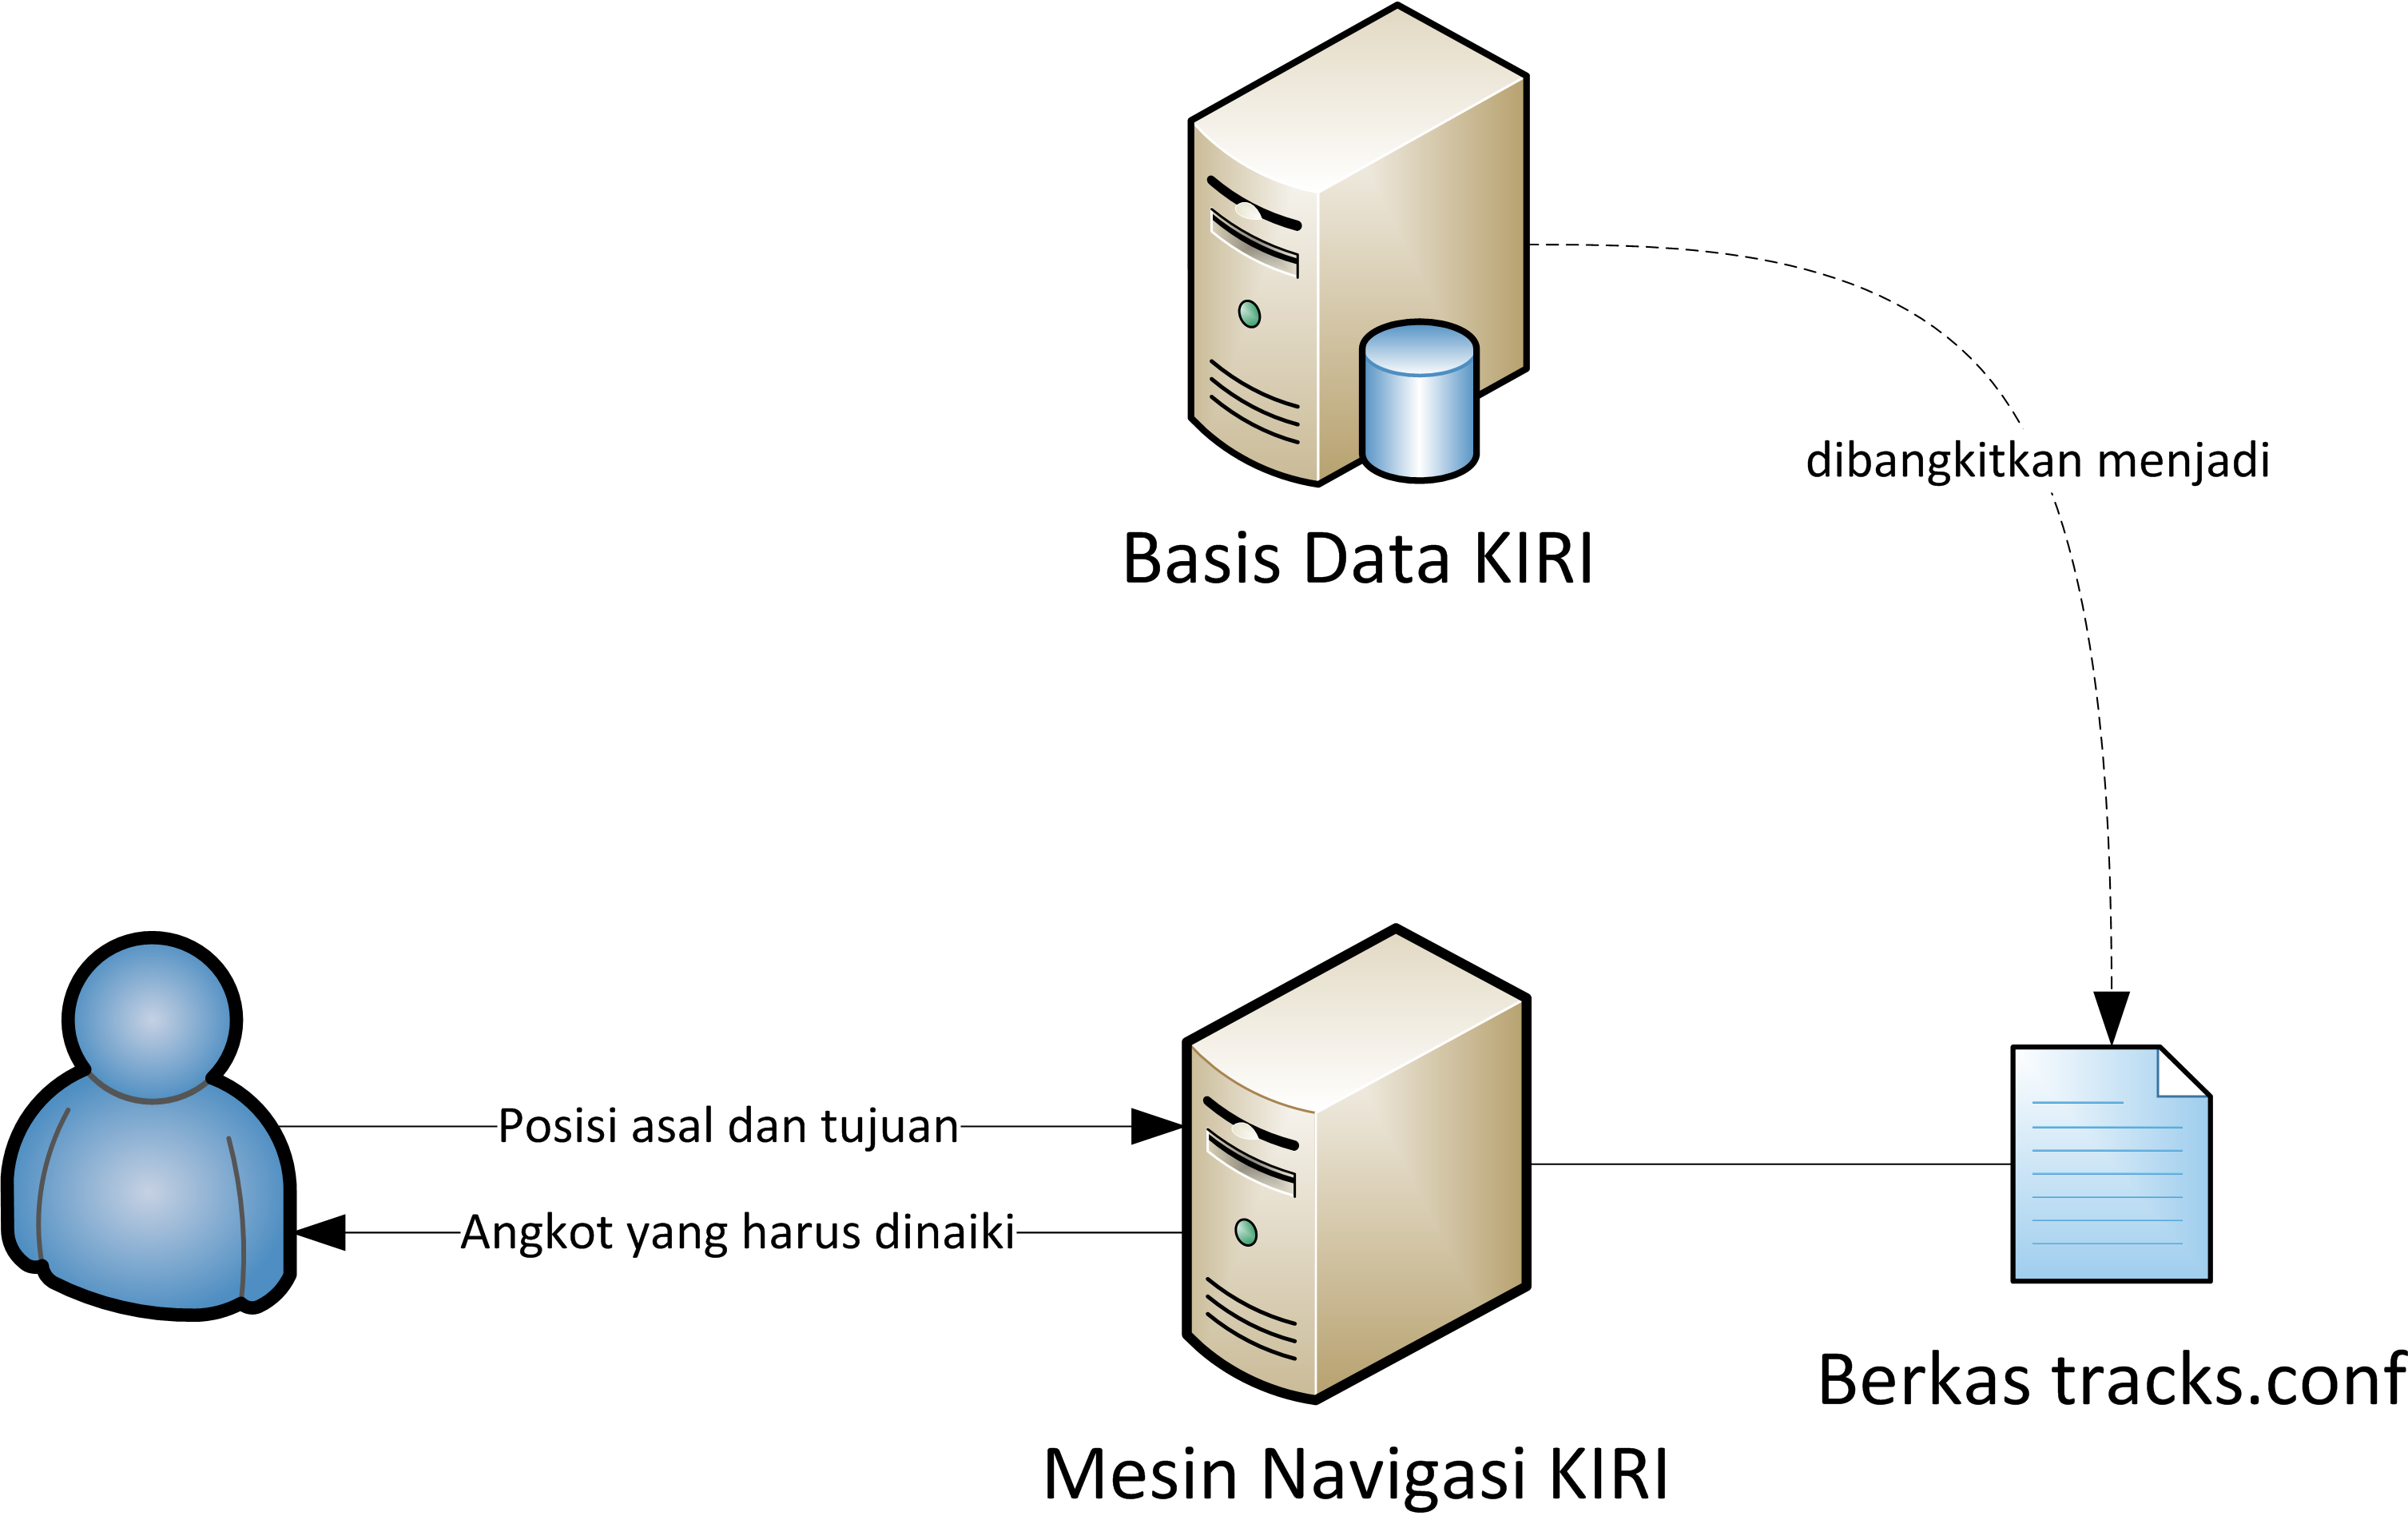
\includegraphics[scale=0.7]{Gambar/2_arsitektur_saat_ini}
	\caption{Arsitektur Saat Ini} 
	\label{fig:2_arsitektur_saat_ini}
\end{figure}

Seperti dapat dilihat pada gambar \ref{fig:2_arsitektur_saat_ini}, elemen
arsitektur yang mendukung navigasi KIRI dibagi menjadi tiga, yaitu:

\begin{enumerate}
	\item \textbf{Basis Data KIRI} menyimpan informasi rute 33 trayek angkot, yang masing-masing mencakup identifikasi trayek (\texttt{trackId} dan \texttt{trackTypeId}), nama trayek (\texttt{trackName}), daftar koordinat yang dilewati (\texttt{geodata}), informasi pulang-pergi (\texttt{pathloop}), catatan internal (\texttt{internalInfo}), prioritas untuk dipilih (\texttt{penalty}), informasi naik/turun penumpang (\texttt{transferNodes}), dan parameter ekstra untuk pembelian tiket (\texttt{extraParameters}).
	\item \textbf{Berkas tracks.conf} adalah hasil ekstraksi dari basis data KIRI, yang menyimpan informasi penting saja yang dibutuhkan oleh algoritma mesin navigasi KIRI, yakni: \texttt{trackId}, \texttt{trackTypeId}, \texttt{penalty}, \texttt{geodata}, \texttt{pathloop}, dan \texttt{transferNodes}.
	\item \textbf{Mesin Navigasi KIRI} adalah program yang bertugas mengolah data yang ada pada berkas tracks.conf, sehingga dapat menjawab pertanyaan navigasi dari titik asal ke titik tujuan. Karena alasan historis, mesin navigasi tidak membaca data langsung dari basis data, melainkan dari berkas tracks.conf.
\end{enumerate}

Ketiga elemen tersebut dijelaskan pada subbab-subbab berikut.

\subsection{Basis Data KIRI}
Basis data KIRI disimpan dalam sistem manajemen basis data MySQL. Salah satu dari tabel yang digunakan adalah tabel \texttt{tracks}, yang menyimpan informasi rute trayek. Struktur dari tabel ini dijelaskan pada tabel \ref{tab:2_struktur_tabel_tracks}.

\begin{table}
	\caption{Struktur Tabel tracks}
	\label{tab:2_struktur_tabel_tracks}
	\begin{tabular}{|p{3cm}|p{2.5cm}|p{9.5cm}|}
		\hline
		Nama kolom & Tipe & Keterangan \\
		\hline
		trackId & varchar(32) & Kode trayek angkot (misal: ``\texttt{sthallciumbuleuitlurus}''). Menjadi PRIMARY KEY tabel bersama trackTypeId. \\
		trackTypeId & varchar(32) & Kode tipe trayek (untuk angkot bandung, selalu berisi ``\texttt{bdo\_angkot}''). Menjadi PRIMARY KEY bersama trackId. \\
		trackName & varchar(32) & Nama trayek yang dapat dibaca secara umum (misal: ``\texttt{St. Hall - Ciumbuleuit (lurus)}''). \\
		internalInfo & varchar(1024) & Informasi internal yang dapat ditambahkan dan tidak akan ditampilkan pada hasil pencarian. \\
		geodata & linestring & Daftar koordinat dari rute trayek ini. \\
		pathloop & tinyint(1) & Menandakan apakah trayek ini adalah trayek pulang pergi atau satu arah. \\
		penalty & decimal(4,2) & Bobot dari trayek ini. Semakin besar nilainya, semakin kecil kemungkinan akan muncul pada hasil navigasi. \\
		transferNodes & varchar(1024) & Daftar indeks titik di mana penumpang dapat turun maupun naik, dipisahkan dengan koma. Untuk angkot Bandung, penumpang dapat turun dan naik di semua titik. \\
		extraParameters & varchar(256) & Informasi yang ditambahkan saat melakukan pembelian tiket (tidak terkait dengan penelitian ini). \\
		\hline
	\end{tabular}
\end{table}

\subsection{Berkas tracks.conf}
Karena alasan historis\footnote{Pada awalnya mesin navigasi KIRI dibangun menggunakan bahasa C++, sehingga menyulitkan dalam mengakses basis data MySQL}, mesin navigasi KIRI tidak mengakses langsung ke basis data MySQL, melainkan membaca sebuah berkas yang bernama \texttt{tracks.conf}.

Berkas \texttt{tracks.conf} ini merupakan sebuah berkas teks yang menyimpan basis data trayek yang telah dibersihkan untuk dapat dibaca dengan mudah, satu \textit{record} per baris. Setiap baris berisi 6 \textit{field} yang dipisahkan dengan \textit{tab} (\textit{Unicode} U+0009\cite{unicode8}). Berikut adalah penjelasan dari keenam \textit{field} tersebut:

\begin{enumerate}
	\item \textbf{trackTypeId.trackId} Berisi \texttt{trackTypeId} dan \texttt{trackId} dipisahkan dengan titik.
	\item \textbf{penalty} Berisi nilai \texttt{penalty}.
	\item \textbf{numberOfNodes} Berisi jumlah \textit{node} (titik) dari rute trayek ini.
	\item \textbf{nodes} Berisi daftar koordinat \textit{node} dari rute trayek ini dipisahkan dengan \textit{tab}. Setiap koordinat node terdiri dari \textit{latitude} dan \textit{longitude} yang dipisahkan dengan spasi.
	\item \textbf{pathLoop} Berisi nilai \texttt{pathloop} yang menunjukkan apakah rute ini merupakan rute pulang pergi atau searah.
	\item \textbf{transferNodes} Berisi nilai \texttt{transferNodes} yang menunjukkan titik-titik di mana penumpang diperbolehkan untuk naik / turun.
\end{enumerate}

\subsection{Mesin Navigasi KIRI}

Mesin navigasi KIRI merupakan sebuah program yang mendengarkan dan menjawab permintaan navigasi dalam bentuk \textit{HTTP request} di \textit{port} 8000. Program ini dibangun di atas bahasa Java, yang terdiri dari beberapa kelas yang ditunjukkan pada gambar \ref{fig:2_diagram_kelas_sistem_kini}.

\begin{figure}
	\centering
	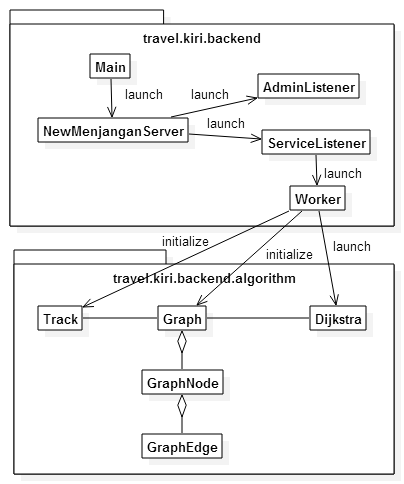
\includegraphics[scale=0.5]{Gambar/2_diagram_kelas_sistem_kini}
	\caption{Diagram Kelas Sistem Kini} 
	\label{fig:2_diagram_kelas_sistem_kini}
\end{figure}

Adapun penjelasan untuk setiap kelas dapat dilihat di bawah ini:

\begin{description}
	\item[Main] Kelas yang berfungsi sebagai antarmuka program, untuk dijalankan dari \textit{console}.
	\item[NewMenjanganServer] Kelas yang bertugas menjalankan program sebagai server, yakni menyiapkan servis-servis untuk dijalankan.
	\item[AdminListener] Kelas yang berfungsi untuk mendengarkan dan merespon perintah administrasi, seperti \textit{ping}, \textit{shutdown}, dll.
	\item[ServiceListener] Kelas yang berfungsi untuk mendengarkan dan merespon permintaan untuk navigasi. Servis ini menerima masukan berupa koordinat asal dan tujuan, dan mengembalikan rute angkot yang harus dinaiki.
	\item[Worker] Kelas ini berfungsi untuk melakukan pekerjaan yang telah diterima oleh ServiceListener. Selain itu, di awal kelas ini juga menyiapkan bahan-bahan yang diperlukan untuk melakukan perhitungan rute, yakni mengkonversi data trayek ke dalam bentuk graf.
	\item[Track] Kelas ini berfungsi untuk menyimpan informasi sebuah trayek angkot beserta rutenya.
	\item[Graph] Kelas ini merepresentasikan sebuah graf.
	\item[GraphNode] Kelas ini merepresentasikan setiap \textit{node} yang dimiliki oleh graf.
	\item[GraphEdge] Kelas ini merepresentasikan sebuah \textit{edge} dari GraphNode.
	\item[Dijkstra] Kelas ini merepresentasikan algoritma \textit{Dijkstra's shortest path}\cite{Cormen:2001}, untuk digunakan dalam pencarian rute.
\end{description}

\section{Protokol Peta Angkutan Umum}

Berdasarkan kode sumber Peta Angkutan Umum \cite{angkotwebid}, situs tersebut memanfaatkan \textit{HTTP request} \cite{rfc7231} untuk menerima perintah-perintah dan mengembalikan respon berupa data dalam sintaks JSON. Beberapa dari perintah tersebut dijelaskan pada subbab-subbab berikut.

\subsection{Transportation List}
Perintah ini digunakan untuk mendapatkan daftar semua daftar transportasi umum, dan dapat diakses pada dengan melakukan \textit{HTTP request GET} pada path \texttt{/route/transportation-list.json}, tanpa parameter apapun. Adapun kembalian dari perintah ini adalah sebuah objek JSON yang terdiri dari pasangan nama/nilai berikut:

\begin{itemize}
	\item \texttt{status}: Status kembalian dari perintah yang dikirimkan
	\item \texttt{provinces}: \textit{Array} provinsi yang terdaftar, masing-masing elemen merupakan \textit{array} lain yang berisi:
		\begin{itemize}
			\item Kode provinsi
			\item Nama provinsi
		\end{itemize}
	\item \texttt{transportations}: \textit{Array} provinsi yang terdaftar, masing-masing berisi:
		\begin{itemize}
			\item \texttt{hasroute}: Menyatakan apakah trayek ini memiliki data rute
			\item \texttt{company}: Perusahaan pengelola trayek ini
			\item \texttt{id}: Indeks trayek ini dalam basis data
			\item \texttt{origin}: Awal rute trayek
			\item \texttt{destination}: Akhir rute trayek
			\item \texttt{province}: Provinsi tempat trayek ini beroperasi
			\item \texttt{city}: Kota tempat trayek ini beroperasi
			\item \texttt{number}: Nomer trayek
			\item \texttt{created}: \textit{UNIX time} trayek ini dibuat
			\item \texttt{updated}: \textit{UNIX time} trayek ini terakhir diperbaharui
		\end{itemize}
\end{itemize}

Contoh kembalian dari perintah transportation list (\url{https://angkot.web.id/route/transportation-list.json}) dapat dilihat pada kode di bawah ini:

\begin{lstlisting}
{
	"status": "ok",
	"provinces": [
		[
			"ID-AC",
			"Aceh"
		],
		...
	],
	"transportations": [
		{
			"hasRoute": true,
			"company": "KWK",
			"id": 21,
			"origin": null,
			"destination": null,
			"province": "ID-JK",
			"city": "Jakarta",
			"number": "S15A",
			"created": "1379952348",
			"updated": "1379952379"
		},
		...
	]
}
\end{lstlisting}

\subsection{Transportation Detail}
Perintah ini digunakan untuk mendapatkan detail dari sebuah trayek transportasi, dan diakses dengan melakukan \textit{HTTP request GET} pada path \texttt{/route/transportation/nnn.json} (di mana \textit{nnn} adalah nomer kode trayek dalam basis data). Adapun kembalian dari perintah ini adalah:

\begin{itemize}
	\item \texttt{id}: Nomer kode trayek.
	\item \texttt{geojson}: Data rute dan atributnya dalam format GeoJSON, terdiri dari:
		\begin{itemize}
			\item \texttt{type}: Tipe GeoJSON yang digunakan, selalu berisi ``\texttt{Feature}''
			\item \texttt{properties}: Properti-properti data GeoJSON, terdiri dari:
				\begin{itemize}
					\item \texttt{number}: Nomer trayek
					\item \texttt{accept}: \textit{tidak diketahui}
					\item \texttt{company}: Perusahaan pengelola trayek ini
					\item \texttt{destination}: Akhir rute trayek
					\item \texttt{province}: Provisi tempat trayek ini beroperasi
					\item \texttt{origin}: Awal rute trayek
					\item \texttt{city}: Kote tempat trayek ini beroperasi
				\end{itemize}
			\item \texttt{properties}: Data geometri rute trayek ini, mengikuti standar GeoJSON untuk tipe data \texttt{MultiLineString}.
		\end{itemize}
	\item \texttt{created}: \textit{UNIX time} trayek ini dibuat
	\item \texttt{status}: Status kembalian dari perintah yang dikirimkan
	\item \texttt{submission\_id}: Kode submisi dari trayek yang dimaksud
	\item \texttt{updated}: \textit{UNIX time} trayek ini terakhir diperbaharui
\end{itemize}

Contoh kembalian dari perintah transportation (https://angkot.web.id/route/transportation/348.json) dapat dilihat pada kode berikut:

\begin{lstlisting}
{
	"id": 348,
	"geojson": {
		"type": "Feature",
		"properties": {
			"number": "M24v2",
			"accept": [],
			"company": "Mikrolet",
			"destination": "Joglo",
			"province": "ID-JK",
			"origin": "Terminal Grogol",
			"city": "Jakarta"
		},
		"geometry": {
			"type": "MultiLineString",
			"coordinates": [
				[
					[106.79068207740782, -6.166144969433212],
					[106.79347157478333, -6.166107635752627],
					[106.79707646369934, -6.165899633769797],
					...
				],
				[
					[106.7961323261261, -6.196021736671819],
					[106.7957353591919, -6.196037735916297],
					[106.79550468921661, -6.195936407359816],
					...
				]
			]
		}
	},
	"created": "1402504737",
	"status": "ok",
	"submission_id": "CaZVRi",
	"updated": "1402506397"
}
\end{lstlisting}
